\documentclass[dutch, twoside, a4paper, 10pt]{article}
\usepackage[utf8]{inputenc}
\usepackage{float}
\usepackage{babel}
\usepackage{graphicx}
\usepackage{geometry}
\usepackage{wrapfig}
\usepackage{caption}
\usepackage{fancyhdr}
\usepackage{fontspec}

\usepackage{hyperref}
\urlstyle{same}

\usepackage{titlesec}
\titlespacing{\section}{0pt}{*4}{*1.5}

\linespread{1.15}

\geometry{
 a4paper,
 left=25mm,
 top=15mm,
 }
\setromanfont{Verdana}


\title{\vspace{75mm}In welke mate is AI in staat muziek te genereren op basis van bladmuziek? \\[1ex] \large Tsj-AI-kovski }
\author{\small Arthur Van Loo 6D2-C 7\\ \small Sint-Franciscus-Xaveriusinstituut}
\date{ \vspace{-5mm} \small 2021-2022}

\renewcommand\headrulewidth{0pt} % no line between document and header
\fancyhead{} % clear header
\fancyfoot{} % clear footer
\fancyfoot[EL,RO]{\thepage}
\pagestyle{fancy}

\begin{document}

\LARGE \maketitle
\thispagestyle{empty}
\newpage
\mbox{}
\newpage
\normalsize

\tableofcontents

\newpage

\section{Inleiding}
\noindent
Zoals uit de titel afgeleid kan worden, werd in dit onderzoek artificiële intelligentie gebruikt. Dit is een ruim begrip voor alle intelligentie die door de mens gemaakt is. Dit kan alles omvatten van beslissingsbomen tot neurale netwerken. Dit laatste type is gebaseerd op biologische, neurale netwerken en ook daarvan bestaan er veel variëteiten. Deze varianten kunnen verschillende taken uitvoeren: visuele herkenning, regressieanalyse, enzovoort. Aangezien er in dit vakgebied heel wat jargon voorkomt, werd de uitleg beperkt tot essentiële termen. Voor drie andere termen wordt wel een verwijzing aangeboden met aanvullende informatie.
\par\bigskip\noindent
Bij dit experiment werd een GAN (Generative Adversarial Networks) gebruikt. Dit systeem bestaat uit twee neurale netwerken: de generator en de discriminator. De eerste, de generator, kan het best vergeleken worden met een kunstvervalser. De discriminator is dan een kunstveiler.  De eerste presenteert zijn schilderijen als authentieke stukken om zo veel geld te verdienen. De veiler wil uiteraard zijn reputatie niet schaden. Stel dat de vervalser zich enkel focust op het werk van Picasso. Als hij nog geen enkele Picasso's bestudeerd heeft, zal dit niet goed lukken. Een kunstveiler zonder ervaring zal ook willekeurig moeten beslissen of hij te maken heeft met een echte Picasso of niet. 
\par\bigskip\noindent
Na verloop van tijd worden beiden beter in hun respectievelijke taak: de generator in het produceren en de discriminator in het onderscheiden. Dit principe is ook toepasbaar op de neurale netwerken. Aan de hand van een algoritme worden de parameters steeds nauwkeuriger afgestemt. Tegenwoordig zijn GAN's vrij geoptimaliseerd. Dit soort structuren wordt gebruikt voor alles wat geproduceerd kan worden (vandaar \textit{Generative}): afbeeldingen van gezichten, menselijke stemmen en zelfs kunst.
% De eerste, de generator, kijkt naar de verzamelde dataset en probeert gelijkaardige afbeeldingen te produceren. De discriminator, ook wel de inspecteur, probeert de namaak-afbeeldingen te onderscheiden van de originele. In het begin gebeurt dit willekeurig (cf. de \textit{gewichten} van de synapsen zijn nog willekeurig). Na verloop van tijd worden beide netwerken beter. 

\begin{figure}[h!]
    \centering
    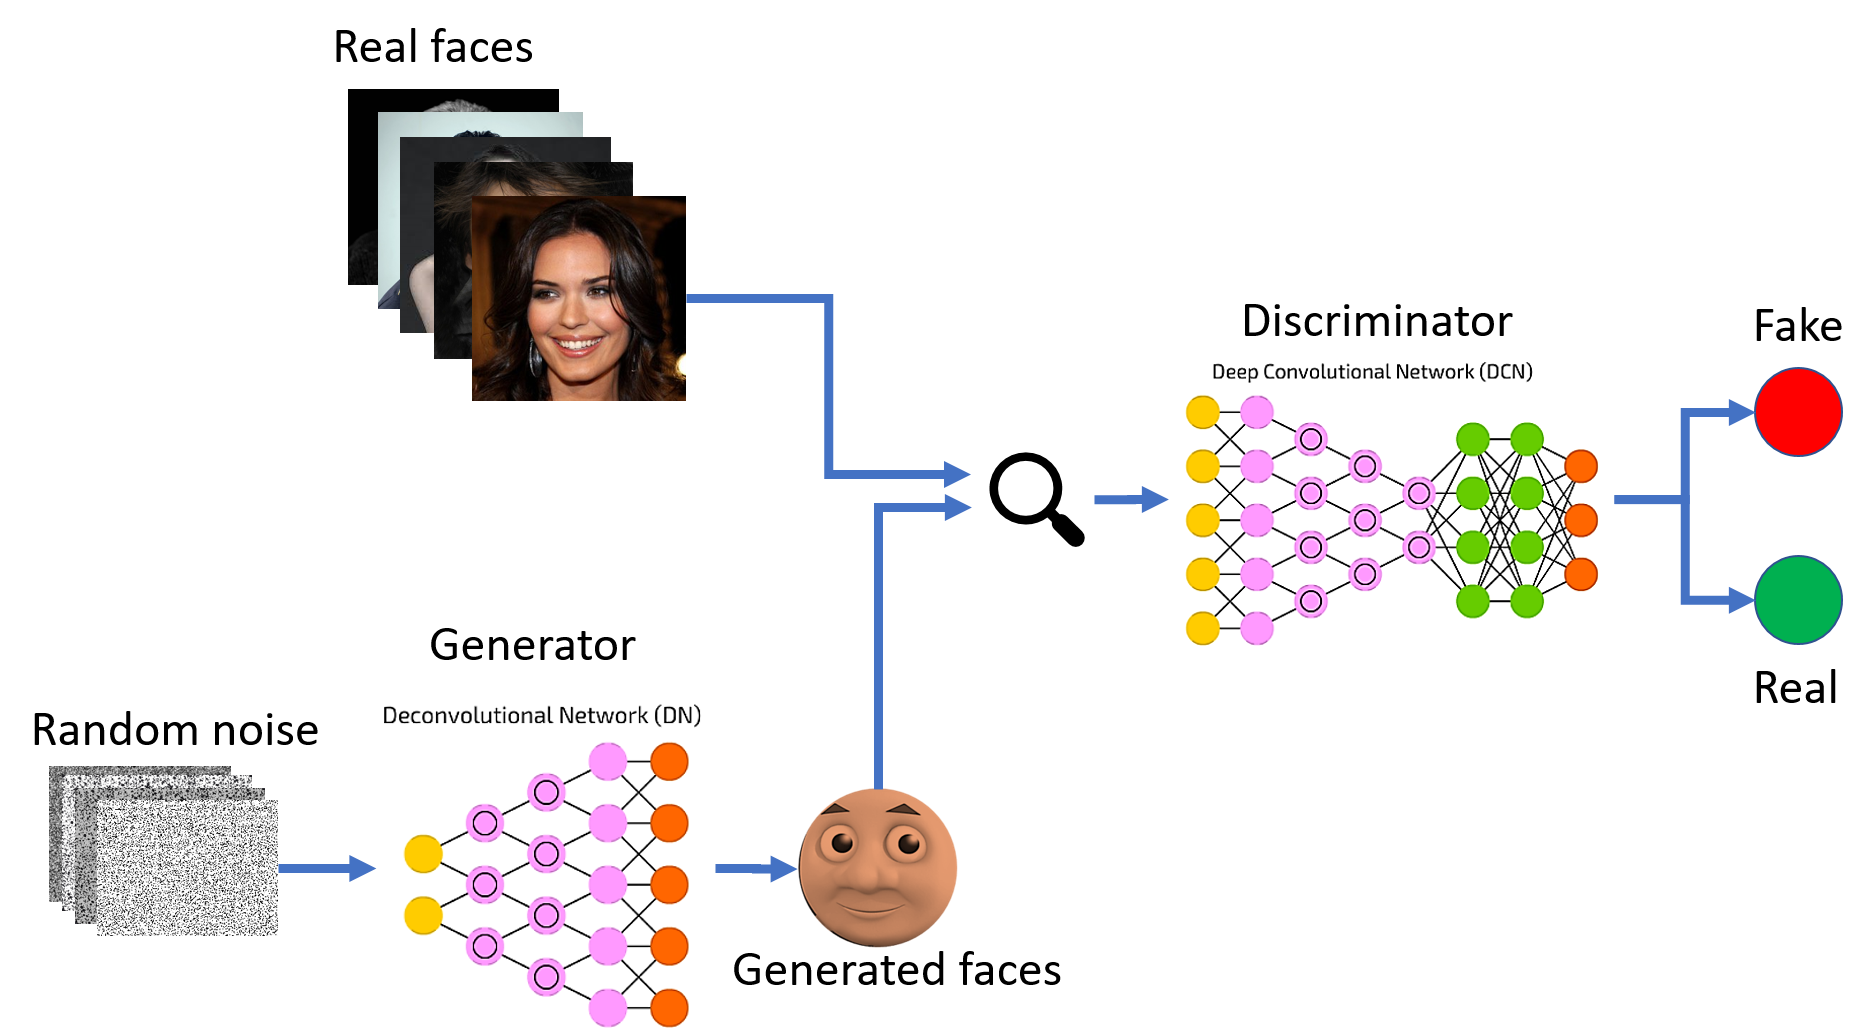
\includegraphics[scale=0.25]{GAN_en.png}
    % \captionsetup{labelformat=empty}
    \caption{Structuur GAN}
\end{figure}

\begin{wrapfigure}{r}{0.33\textwidth}
    \vspace{-\baselineskip}
    \centering
    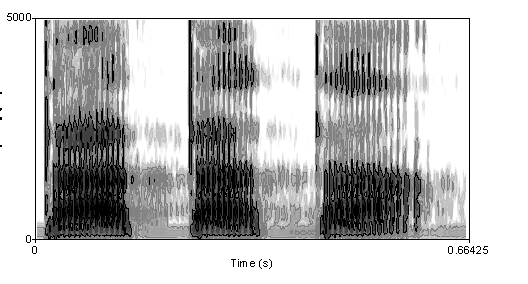
\includegraphics[width=0.33\textwidth, trim={2 0 0 0}, clip]{Praat-spectrogram-tatata.png}
    \caption{Spectrogram}
    \label{fig:Spectrogram}
    
    \vspace{-3\baselineskip}
\end{wrapfigure}
\noindent
In heel wat domeinen wordt AI gebruikt om het leven van de mens beter en eenvoudiger te maken. Het is bovendien al meermaals aangetoond dat GAN's ook muziek kunnen produceren. Dit gebeurt meestal via spectrogrammen (een weergave van de frequentie in functie van de tijd; zie figuur \ref{fig:Spectrogram}). Hiervoor is echter een extra berekeningsstap\footnote{\url{https://nl.wikipedia.org/wiki/Fast_Fourier_transform}} nodig. De vraag die dan vanzelf opkomt is of we een stap kunnen terugkeren. Kunnen GAN's ook partituren produceren? Zo ja, hoe goed of hoe creatief zijn ze daarin? Een mogelijke hypothese is dat de netwerken herhaalde structuren (notenbalken, noten en maatstrepen) zonder veel moeite kunnen reproduceren. Partituren die leesbaar zijn voor de mens zullen vermoedelijk niet verkregen worden. Als we de resultaten van particuliere GAN-projecten bekijken, treden gelijkaardige verschijnselen op: de algemene vorm van een object wordt herkend. Details komen in de praktijk enkel voor in systemen die door grote bedrijven (o.a. DeepMind en OpenAI) vervaardigd zijn. 
\par\bigskip\noindent
Een alternatieve naam voor dit onderzoek is Tsj-AI-kovski. Tsjaikovski is een bekende, Russische componist. De \textit{ai} in diens naam kan staan voor artificiële intelligentie.

\section{Materiaal}

\begin{itemize}
\setlength{\itemsep}{1pt}
\item Dell Inspiron 15 Plus, Intel i5 CPU, 16GB RAM, 512GB SSD
\item Internetverbinding
\item NVIDIA GPU (GTX 1650)
\item \textit{Lightweight GAN} broncode
\end{itemize}
Vermits het hier om een project gaat met artificiële intelligentie, hebben we uiteraard een computer met toegang tot het internet nodig. GAN's bestaan zoals eerder vermeld uit twee neurale netwerken. Dit betekent dat het trainen meer rekenkracht vereist dan bij enkele netwerken. Dit wijst meteen op het belang van grafische kaarten of GPU's. In dit geval werd gebruikgemaakt van NVIDIA's GTX 1650. \par\bigskip\noindent
Een andere vereiste is een groot aantal afbeeldingen. Deze dienen als studiemateriaal voor de generator en als controle voor de discriminator. Aangezien veel grote componisten reeds lang geleden het leven lieten, behoort hun werk tot het publieke domein. Bijgevolg kunnen hun partituren eenvoudig teruggevonden worden op het internet. Ten slotte stelt dit onderzoek zich niet tot doel het wiel opnieuw uit te vinden. Daarom wordt gebruikgemaakt van een gepubliceerd model op GitHub. GitHub is de grootste verzameling van opensourceprojecten (publiek-beschikbare code).  Broncode die daar te vinden is, bepaalt automatisch structuur (o.a. het aantal neuronen per laag) en zorgt voor een toegankelijk interface. Hierdoor kan men meteen het netwerk trainen en de resultaten analyseren. In het volgende onderdeel wordt hier dieper op ingegaan.

\section{Methode}
\subsection{Dataset verzamelen}
De basis van elk AI-project is een goede dataset. OMR-Datasets (\url{https://apacha.github.io/OMR-Datasets/}) is een verzameling van verschillende, muzikale datasets. De meeste daarvan bevatten naast afbeeldingen ook aanduidingen waar de noten (en andere interessante structuren) zich bevinden. Aanvankelijk leek dit een goede bron, maar bij nader inzien voldeed slechts twee van de verwijzingen aan de eisen van het onderzoek: PrIMuS en IMSLP (\url{https://imslp.org}). De eerste vertoonde veel onnodige informatie en moest nog verder geordend worden voor dit project. Om die redenen genoot IMSLP de voorkeur. Op die webpagina kunnen particulieren zonder extra kosten PDF-bestanden van bladmuziek downloaden. 
\subsection{Dataset schoonmaken} 
Voor het onderzoek is het gewenst \textit{schone data} te gebruiken. Dit wil zeggen dat er zich zo weinig mogelijk randinformatie in de data mag bevinden. Pianomuziek leek hiervoor het best, omdat er relatief veel pianomuziek zonder neveninformatie bestaat. Bovendien moesten de partituren uit wit papier bestaan en geen inktvlekken bevatten. Het netwerk zou anders afgeleid kunnen worden door die uitzonderingen. Dit alles resulteert in het feit dat het verzamelproces niet geautomatiseerd kan worden. Gezien de structuur van IMSLP konden de bestanden toch vrij gemakkelijk gecontroleerd en gedownload worden.
\par\bigskip\noindent
Nadat voldoende PDF-documenten verzameld waren (340 in totaal), werden ze eerst per pagina gesplitst. Hiervoor werd Apple's \textit{Automator} programma gebruikt. Vervolgens werden deze pagina's per notenbalk gesplitst. Hiervoor werd \textit{Chen and Sim's SmartCropper} gebruikt bovenop eigen Python code om het proces te automatiseren en de afbeeldingen gestructureerd te hernoemen. Hieruit werden 1651 foto's verkregen. De splitsing levert niet alleen meer data op maar bovendien zullen er minder details verloren gaan. De afbeeldingen moesten namelijk nog eens verkleind worden naar 256 bij 256 pixels. De verklaring hiervoor is simpel: hoe groter het aantal pixels, hoe groter het aantal parameters je netwerk zal bevatten. Dit laatste betekent langere trainingstijden en een grotere tol op de rekenkracht. 
\par\bigskip\noindent
De vierkante afbeeldingen kunnen verklaard worden aan de hand van de broncode. De afbeeldingen bestaan zoals reeds vermeld uit pixels. Deze worden gelezen als een tensor\footnote{\url{https://nl.wikipedia.org/wiki/Tensor}} van 3 keer 65.536 pixels. Daarna wordt die tensor `uitgevlakt' tot een matrix. Gezien het belang van matrix-operaties in het trainen, is het zowel veilig als eenvoudig om met vierkante matrices te werken. Daaruit volgt dat publieke broncode meestal gebruikt maakt van vierkante afbeeldingen. Dit kan weliswaar aangepast worden, maar daardoor zou kostbare tijd verloren gaan.

\subsection{Het model}
Zoals in titel 2 reeds werd vermeld, is het zinloos (voor dit onderzoek) om de structuur van de netwerken zelf te programmeren. Op het internet (met name op GitHub) zijn diverse modellen gepubliceerd. Deze herbergen alle algoritmes die moeten verlopen opdat de modellen correct en efficiënt kunnen werken.\par\bigskip\noindent
Aanvankelijk leek \textit{StyleGAN2} de beste keuze. Deze toepassing werd enige jaren geleden (2019) gepubliceerd en brengt indrukwekkende resultaten voort. Dusdanige voorbeelden spreken onmiddellijk tot de verbeelding. Desondanks bleek het na verder onderzoek te zwaar voor de beschikbare computertoestellen. Ook \textit{HyperGAN} was te veeleisend en bovendien enigszins verouderd. Ten slotte scheen \textit{Lightweight GAN} alle nodige kenmerken te vertonen. Op het internet zijn er verschillende voorbeelden waar deze broncode op een succesvolle manier toegepast wordt. Het volstaat om de Python programmeertaal te installeren en \textit{pip install lightweight-gan} in een computerterminal in te geven om \textit{Lightweight GAN} lokaal te verkrijgen.

\section{Resultaten}

\noindent Eenmaal alles is ingesteld kan het netwerk beginnen met trainen. Hierbij voorzien we het programma van verschillende 'argumenten', bijvoorbeeld hoe groot de afbeeldingen zijn en hoe frequent we het model willen opslaan. Deze variabelen worden door de broncode opgeslagen. Het traingsproces zelf gebeurt automatisch. In welbepaalde tijdsintervallen (elke tien stappen, met een 'batch'-grootte\footnote{\url{https://de-vraag.com/nl/71942918}} van 4) krijgen we een beeld van het verlies van beide netwerken. Dankzij een formule weten we met andere woorden hoe 'slecht' de netwerken zijn. De uitleg van deze verliesfuncties valt echter buiten de reikwijdte van deze paper. Op hetzelfde ogenblik worden ook negen afbeeldingen geproduceerd door de generator. Daarvan zijn enkele voorbeelden te zien op pagina 8. Gedurende het hele trainingsproces bleef het verlies van de generator vrij groot. Na acht uur en 3980 stappen werd het trainen beëindigd, omdat er geen vooruitgang meer zichtbaar was in de verkregen afbeeldingen.
\section{Discussie}
\noindent Voor leken kunnen deze resultaten niet zeer goed lijken. Het moet echter geweten zijn dat het verzamelen van een goede dataset het grootste probleem is in de wereld van artificiële intelligentie, op de voet gevolgd door rekenkracht. Gezien de tijdsspanne van dit onderzoek, was het niet mogelijk om de \textit{perfecte} dataset samen te stellen. Vooral het splitsen van de afbeeldingen kostte veel tijd. Eerst moeten de documenten per pagina gesplitst worden en vervolgens nog eens per groep van twee notenbalken. Het programma \textit{SmartCropper} dat werd gebruikt bleek bovendien niet foutloos te werken. Sommige afbeeldingen werden gewoon niet gesplitst. Deze tekortkomingen werden aangevuld met eigen Python code. Dit had zijn weerslag op de planning.
\par\bigskip\noindent
Vrijwel alle informaticaprojecten die werken met bladmuziek doen dit om die partituren om te zetten in MIDI-bestanden. Daarom bevatten de beschikbare datasets veel informatie over de plaatsing van de noten en rusttekens. Uiteraard zouden deze datasets ook voor de desbetreffende taak gebruikt kunnen worden, maar dat zou minstens evenveel werk vereisen als het samenstellen van een eigen archief.
\par\bigskip\noindent
Zelfs als we over een volmaakte dataset zouden beschikken, zou dit geen garantie zijn voor heldere (en misschien zelfs creatieve) bladmuziek. Verschillende andere factoren spelen nog een rol. Zoals eerder vermeld is rekenkracht van belang. GAN's hebben gewoonlijk een halve dag nodig om te trainen. De grafische kaart die in dit onderzoek werd gebruikt (GTX 1650) is zeer efficiënt voor dagelijks tot zwaarder gebruik. Voor AI-projecten liggen de eisen echter veel hoger. Daarom zijn het ook enkel grote bedrijven die met \textit{perfecte} resultaten komen. Tenslotte kan het ook aan de aard van bladmuziek liggen, partituren bevatten namelijk een zeer hoge dichtheid aan informatie. Dankzij diverse afspraken kunnen mensen met enige oefening deze lezen. De computer is zich echter niet bewust van wat hij voorgeschoteld kreeg en welke regels er voor die elementen bestaan. Meer zelfs: hij weet niet of er regels in bestaan.
\par\bigskip\noindent
We kunnen concluderen dat de hypothese vrij goed aansluit bij het eindproduct. We zien de ruggengraat van bladmuziek met noten en notenbalken, maar maatstrepen zijn er niet. Dit ligt vermoedelijk aan het feit dat deze erg verspreid liggen in de dataset. Ook concrete, leesbare afbeeldingen worden niet vervaardigd. 
\newpage
\begin{table}[H]
    \centering
    \caption{Weergave van de resultaten}
    \label{Tab: weergave}
    \begin{tabular}{c p{0.6\linewidth}}
          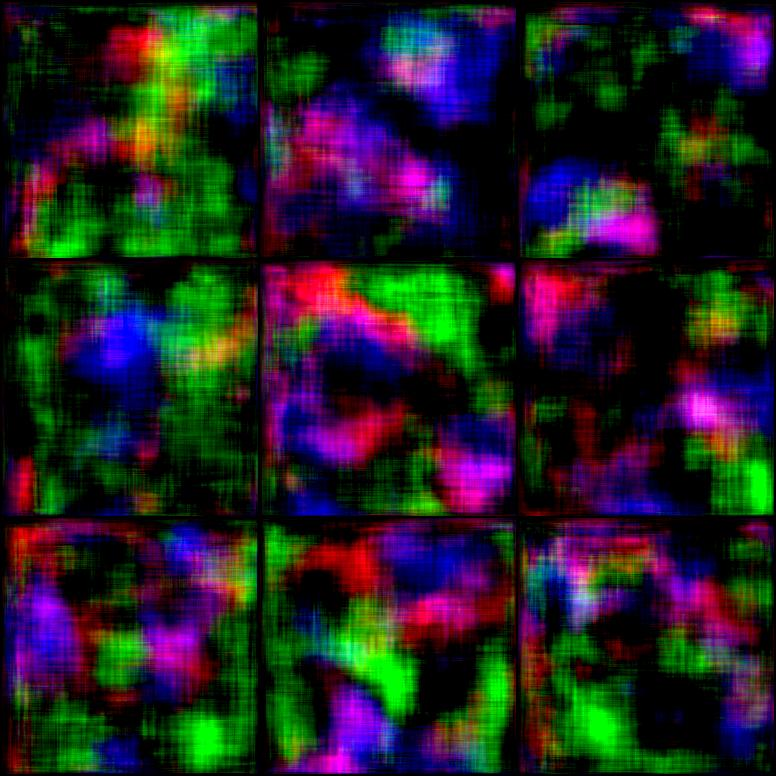
\includegraphics[scale=0.18]{0.jpg}&  \vspace{-10\baselineskip} Dit is de allereerste afbeelding die geproduceerd werd. De afbeelding bestaat voornamelijk uit de kleuren rood, groen, blauw en zwart. Dit is te verwachten. Het netwerk start namelijk met willekeurige parameters. Het gaat hier dus om de 3 hoofdkleuren van computers (RGB) en zwart, die voorgesteld wordt door een nulwaarde.\\
          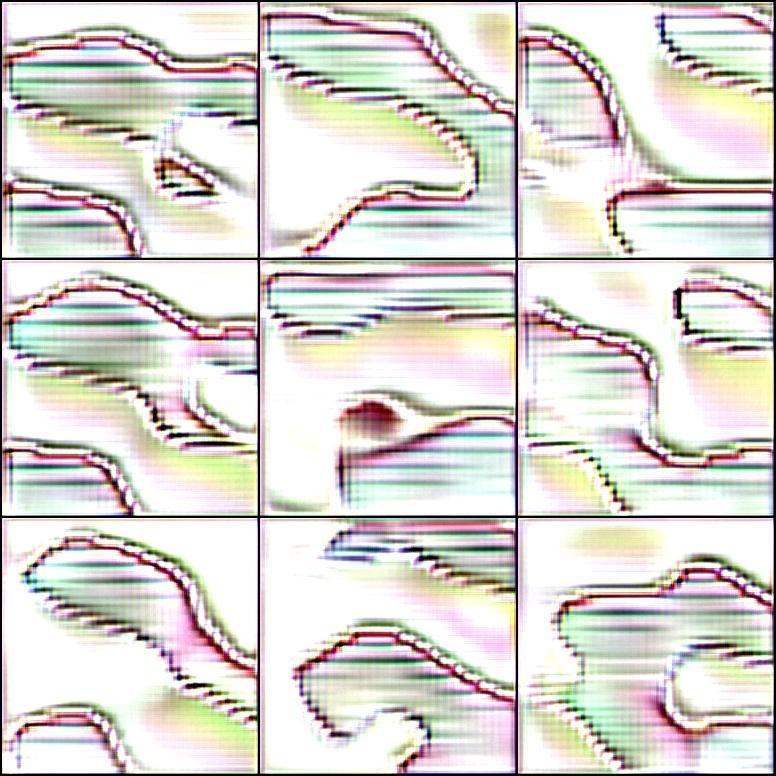
\includegraphics[scale=0.18]{10-interp.jpg}   & \vspace{-10\baselineskip}Vanaf afbeelding 10 zijn er al duidelijk lijnstructuren waar te nemen. Notenbalken bestaan namelijk uit lijnen en die zijn met andere woorden zeer talrijk in de dataset. In onze data bevinden de notenbalken zich niet op dezelfde hoogte; dit uit zich in \textit{(schier)eilanden} van lijnen bij het AI-systeem. \\
          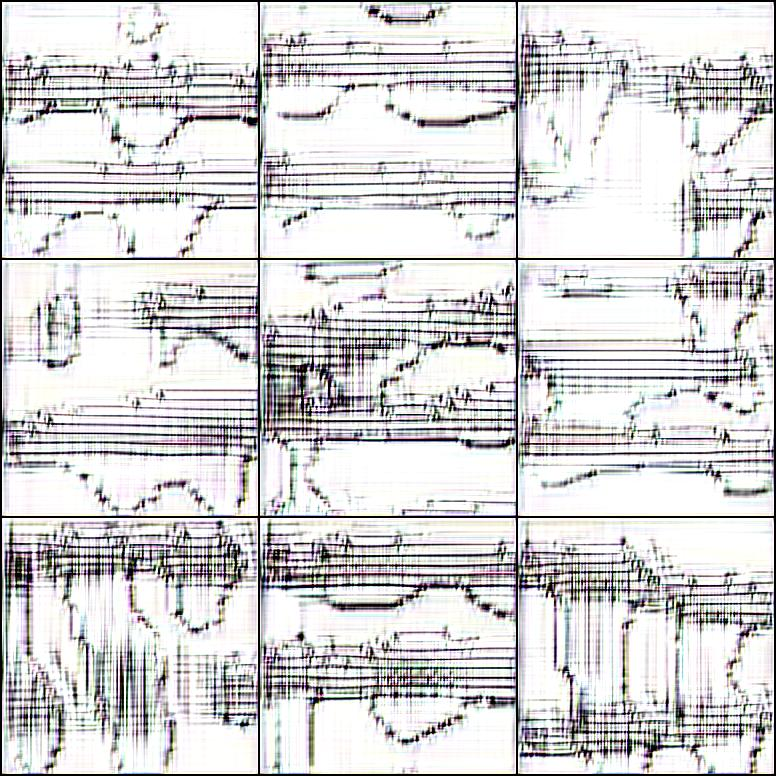
\includegraphics[scale=0.18]{89.jpg} & \vspace{-10\baselineskip} Bij groep 89 is te zien dat de afzonderlijke afbeeldingen vrijwel steeds bestaan uit 2 notenbalken. Daarop zijn structuren terug te vinden die we als de ruggengraat van noten kunnen typeren. \textit{Echte} noten zijn er echter nog niet. Tenslotte is ook de `kleurvervuiling' verdwenen: de afbeeldingen zijn monochroom zoals echte partituren.\\
          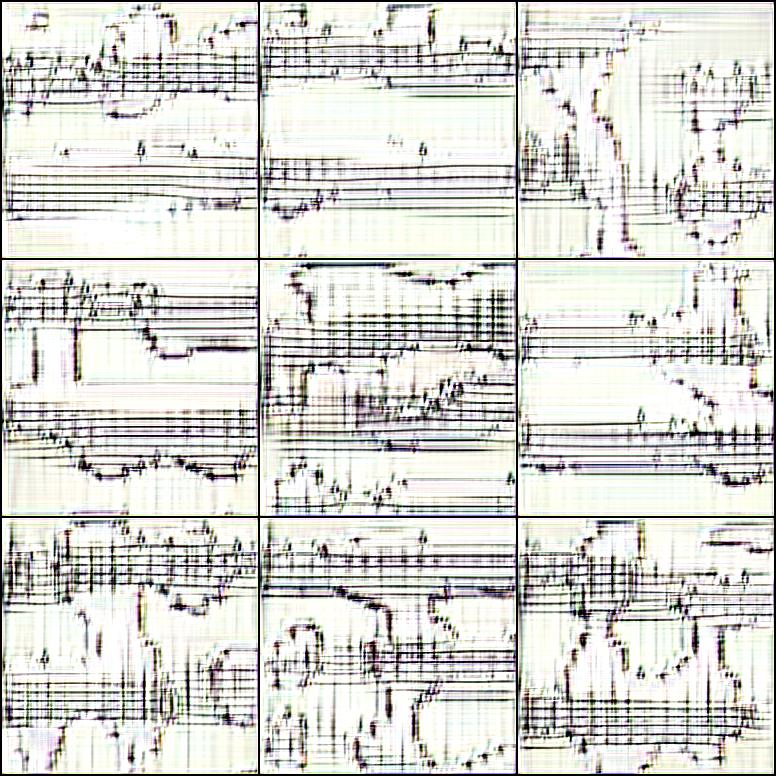
\includegraphics[scale=0.18]{114.jpg}  & \vspace{-10\baselineskip} Bij 114 zijn de afbeeldingen duidelijk scherper en er zijn bijna altijd 5 notenlijnen te vinden. Bovendien zijn er beginsels van akkoorden (bijvoorbeeld in de middelste afbeelding). Een muzikant zou die echter onmogelijk kunnen spelen.\\
          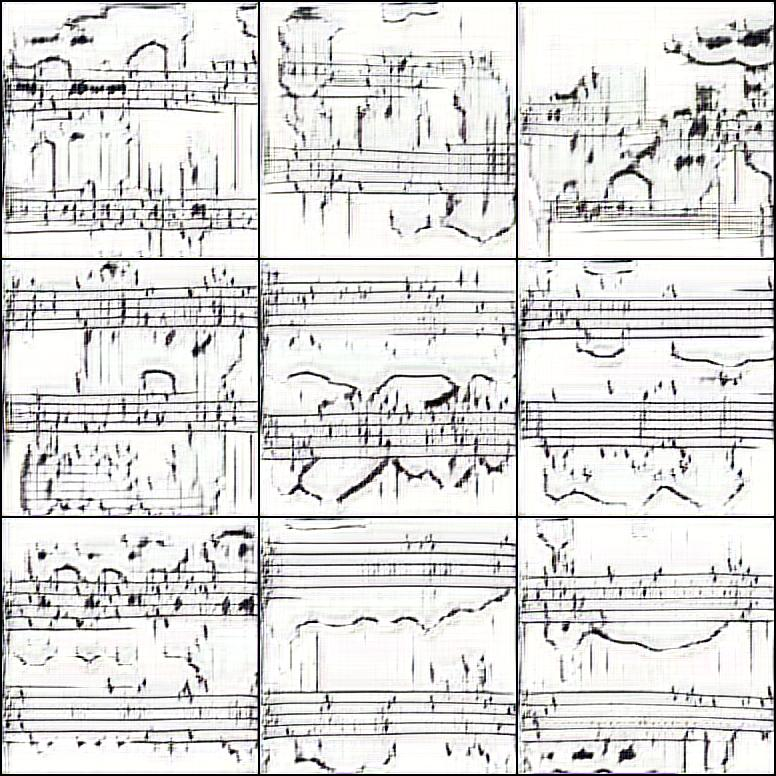
\includegraphics[scale=0.18]{336.jpg}  & \vspace{-10\baselineskip} Bij 336 zijn zowat de beste resultaten terug te vinden. We zien duidelijke noten (die echter niet met de bovenkant verbonden zijn). Notenbalken bestaan zo goed als altijd uit 5 lijnen en aan het begin van elke notenbalk is een vage solsleutel te herkennen. Die is echter zo goed als verdwenen doordat alle afbeeldingen samengedrukt zijn bij het vergaren van de dataset.
    \end{tabular}
\end{table}
\section{Literatuurlijst}
\subsection{Geraadpleegde internetbronnen}
CHEN, W., e.a., \textit{Chen-and-Sim / SmartCropper}. Internet, 21/08/2021, geraadpleegd op 11/05/2022, (\underline{\url{https://github.com/Chen-and-Sim/SmartCropper}})\\
WANG, P., e.a., \textit{lucidrains / lightweight-gan}. Internet, 27/04/2022, geraadpleegd op 11/05/2022,\\ (\underline{\url{https://github.com/lucidrains/lightweight-gan/tree/0.23.2}})
\subsection{Afbeeldingen}
\textit{Generative adversarial networks Artificial neural network Machine learning Artificial intelligence Generative model, Gan, text, media png} [Foto]. (z.d.). PNG EGG. \\ \underline{\url{https://www.pngegg.com/en/png-xflrf}}\\
Maksim (2006, 20 maart). \textit{Praat spectrogram tatata} [Foto]. Wikimedia. \\ \underline{\url{https://commons.wikimedia.org/wiki/File:Praat-spectrogram-tatata.png}}
\section{Logboek}
\renewcommand{\arraystretch}{1.5}
\begin{table}[h!]
\centering
\begin{tabular}{|c|p{0.9\linewidth}|}
    \hline
    23/02 & Formuleren van de onderzoeksvraag; opstellen van een lijst met benodigdheden \\
    \hline
     16/03 & Starten met het maken van de dataset (onderzoek naar diverse, mogelijke bronnen)  \\
     \hline
     30/03 & Dataset afwerken (bestanden downloaden) en \textit{schoonmaken} (afbeeldingen knippen en transformeren naar 256 bij 256 pixels) \\
     \hline
     27/04 & Verkregen data analyseren; beginnen aan verslag en presentatie\\
     \hline
     11/05 & Verslag afwerken (Materiaal en Methode, Resultaten, Discussie en Literatuurlijst); voorbereiden van de presentatie\\
     \hline
\end{tabular}
\end{table}
\end{document}
